%!TEX root = lec16.tex
% ================================================================================
% Lecture 16, Slide 12
% ================================================================================
\begin{frame}[t]
  \mytitle{Inference: Prompting Is Steering}

\begin{columns}[T,totalwidth=\textwidth]

% ------------------------------------------------------------
\begin{column}[T]{0.50\textwidth}
\footnotesize
\vspace{0mm}

\textbf{\textcolor{blue}{A prompt creates the context}}

\vspace{0mm}
\begin{itemize}
  \item system message: role + rules
  \item user message: task + data
  \item the model continues from there
\end{itemize}

\vspace{4mm}
\textbf{\textcolor{red}{Key point:}}
\quad The model is \y{not stable by itself}.  
It is shaped by the context we provide.

\end{column}

% ------------------------------------------------------------
\begin{column}[T]{0.46\textwidth}
\footnotesize
\vspace{0mm}

\textbf{\textcolor{violet}{What improves results}}

\vspace{2mm}
\begin{itemize}
  \item clear goal + constraints
  \item examples of desired style
  \item provide trusted information
  \item ask for uncertainties / checks
\end{itemize}

\vspace{3mm}
{\tiny \textcolor{gray}{
Good prompting is a communication skill:
precise intent, good context, clear quality criteria.
}}
\end{column}

\end{columns}

% ------------------------------------------------------------
% Visualization: prompting = steering (TikZ)
% ------------------------------------------------------------
\vspace{0mm}
\begin{center}
\scalebox{0.85}{
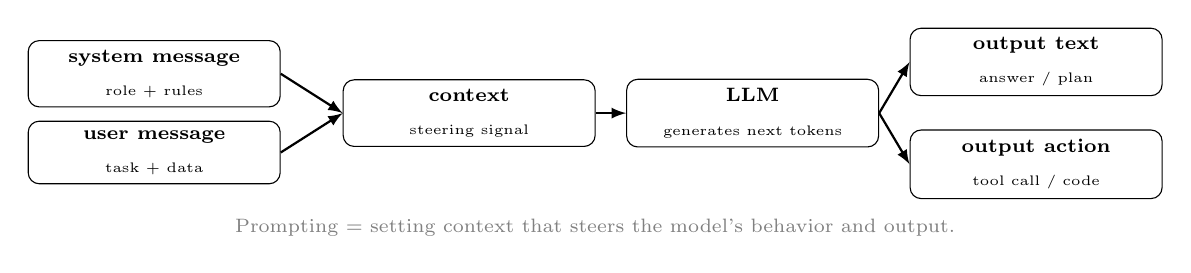
\begin{tikzpicture}[>=latex, x=1cm, y=1cm]

\tikzstyle{box}=[draw, rounded corners, minimum width=3.2cm, minimum height=0.8cm, align=center]
\tikzstyle{smallbox}=[draw, rounded corners, minimum width=3.2cm, minimum height=0.62cm, align=center]
\tikzstyle{arrow}=[->, thick]

% Left: system+user messages
\node[smallbox] (sys) at (-5.0,0.9) {\scriptsize \textbf{system message}\\{\tiny role + rules}};
\node[smallbox] (usr) at (-5.0,-0.1) {\scriptsize \textbf{user message}\\{\tiny task + data}};

% Middle: context / steering
\node[box] (ctx) at (-1.0,0.4) {\scriptsize \textbf{context}\\{\tiny steering signal}};

\draw[arrow] (sys.east) -- (ctx.west);
\draw[arrow] (usr.east) -- (ctx.west);

% Engine: model
\node[box] (llm) at (2.6,0.4) {\scriptsize \textbf{LLM}\\{\tiny generates next tokens}};

\draw[arrow] (ctx.east) -- (llm.west);

% Output
\node[smallbox] (out1) at (6.2,1.05) {\scriptsize \textbf{output text}\\{\tiny answer / plan}};
\node[smallbox] (out2) at (6.2,-0.25) {\scriptsize \textbf{output action}\\{\tiny tool call / code}};

\draw[arrow] (llm.east) -- (out1.west);
\draw[arrow] (llm.east) -- (out2.west);

% Small caption
\node[align=center] at (0.6,-1.05) {\scriptsize \textcolor{gray}{Prompting = setting context that steers the model's behavior and output.}};

\end{tikzpicture}
}
\end{center}

\end{frame}
